\documentclass[11pt]{article}

\title{Proposal for a Guided Research}
\author{Fabian Bell}
\date

\usepackage[english]{babel}
\usepackage{natbib}
\bibliographystyle{abbrvnat}
\setcitestyle{authoryear,open={(},close={)}}
\usepackage{graphicx}
\usepackage{hyperref}

\begin{document}
\maketitle
\section{Background and Motivation}
Dialogue systems (e.g. Chat-bots) have made great progress during the last years. Mainly because of the invention of novel neural models ans machine learning techniques. Because of the progress many current research aims to improve the dialogue systems on a individual and human-like level. Recent article \cite[]{DBLP:journals/corr/abs-1901-08149, liu2020impress} tried to tackle this problem by feeding a persona into the network. The network is then trained to extract characteristic information from the given persona in order to generate a human-like output sequence. The persona is defined by a set of profile sentences like \textit{I like books}. The challenge with these approaches consist of two problems
\begin{itemize}
\item \textbf{Persona understanding:}\\
The network needs to understand what the characteristics of the given persona. This also yields the question on what defines a certain persona and on how formulate the profile sentences, since the Persona definition has to be done manually. 
\item \textbf{Style derivation:}\\
The network needs to derive a certain speaking/writing style from the given persona. Profile sentences like \textit{I bought my first home} \cite[]{liu2020impress} do not necessarily contribute to a distinct writing style.
\end{itemize}
Humans can use various ways of expressing them self, thus it is questionable if the expression style can be defined by just a few sentences. 
\section{Thesis}
Given the previously stated problems one might suggest to rather focus on a single persona and in order to derive a more complex style of writing/speaking. It might also be beneficial to extract the style in a more abstract representation than a persona definition. One possible way of modifying the generation style is pre-training on a biased dataset that contains human generated sequences. \cite[]{wullach2020hate} applied this approach successfully by fine-tuning the the GPT-2 model \cite[]{Radford2019LanguageMA} on a hateful data set in order to modify the generative style without loosing the rich language model encoded in GPT-2. 
This approach could be used for a dialogue system as well. Therefore the thesis of my work is whether additional training on a biased dataset can be used to encode a human-like generative style in a neural network. Further, I will investigate on how to organize the additional training with the original (goal oriented) training. Three possible ways would be \textit{pre-training}, \textit{post-training} or an \textit{interleaved} training procedure. 
\section{Time-line}
\begin{figure}[h]
\centering
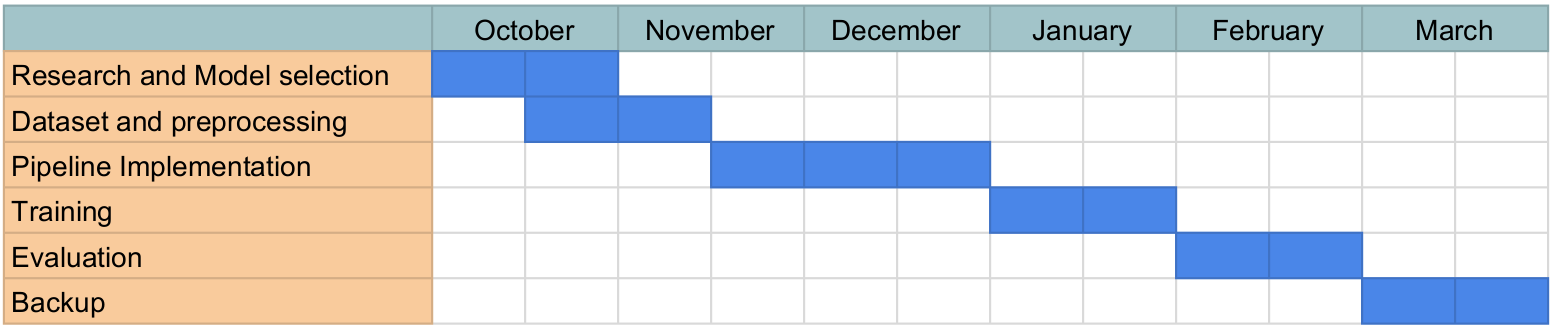
\includegraphics[width=\textwidth]{time-table.png}
\caption{Time-line plan}
\end{figure}

\bibliography{ref}
\end{document}